\section{Durchführung}
\label{sec:Durchführung}

\autoref{fig:aufbau} veranschaulicht den verwendeten Versuchsaufbau.
\begin{figure}
    \centering
    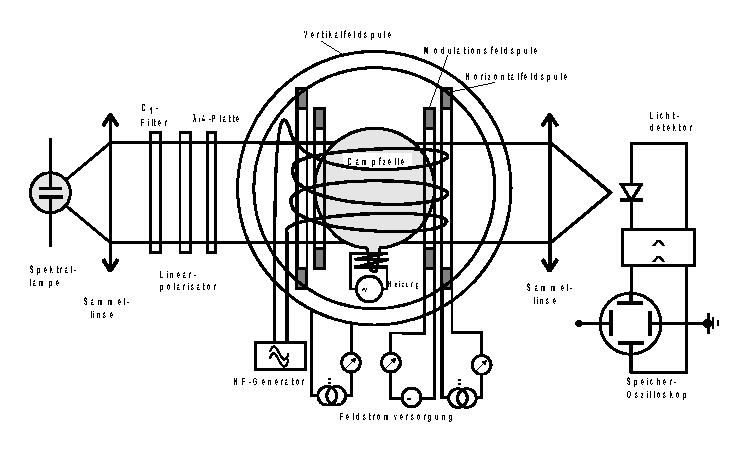
\includegraphics[width=0.95\textwidth]{pictures/Aufbau2.pdf}
    \caption{Schematische Darstellung des verwendeten Versuchaufbaus. \cite{v21}}
    \label{fig:aufbau}
\end{figure} 

Dieser besteht aus einer Rubidiumdampflampe, die Photonen mit der Energie der $D_1$-Linie emittiert. 
Das erzeugte Licht der Wellenlänge $\lambda = \qty{794.8}{nm}$ wird mithilfe einer Linse gebündelt und 
durch Interferenzfilter auf die $D_1$-Komponente reduziert. 
Anschließend wird es durch ein $\lambda/4$-Plättchen zirkular polarisiert. 
Das polarisierte Licht durchläuft eine mit Rubidiumdampf gefüllte Zelle
und wird durch eine weitere Linse fokussiert, um schließlich von einer Photodiode detektiert zu werden. 
Um Dampf zu erzeugen, wird die Rubidiumzelle etwa eine halbe Stunde vor Beginn der Messung auf eine Temperatur von $\SI{50}{\celsius}$ erhitzt.

Die Dampfzelle ist von drei Paaren von Helmholtzspulen umgeben. 
Eine vertikale Spule wird verwendet, um das Erdmagnetfeld auszugleichen, 
während die beiden horizontalen Spulen verwendet werden, um das RF-Feld zu erzeugen. 
Die Ausgabe der Photodiode kann auf einem Oszilloskop im Sweep-Modus angezeigt werden, 
wodurch verschiedene Feldstärken abgedeckt werden können, um präzise Messungen zu ermöglichen. 
Um Umwelteinflüsse zu minimieren, wird der Aufbau nach entsprechender Justierung abgedeckt.

Zu Beginn wird der Versuchsaufbau justiert und der Tisch in Ausrichtung des Erdmagnetfelds positioniert. 
Aufgrund des fehlendem Magnetfeld und der daher sinkenden Transparenz
ist nach Einschalten der Apparatur auf dem Oszilloskop ein Mininum der Durchsichtigkeit zu erkennen.
Durch Anpassung des Vertikalfeldes wird das Erdmagnetfeld kompensiert und der Peak auf dem Oszilloskop sichtbar schmaler. 
Anschließend werden die beiden Rubidiumisotope auf ihre Resonanzstellen untersucht. 
Hierfür wird die RF-Spule aktiviert und Messwerte im Frequenzbereich 
von $\SI{100}{\kilo\hertz}$ bis $\SI{1}{\mega\hertz}$ in Schritten von $\SI{100}{\kilo\hertz}$ aufgezeichnet.
Dabei wird der Sweep-Anteil das horizontale Magnetfeld si variiert,
dass sich die Resonanzstellen auf dem Oszilloskop sichtbar gemacht werden.
